% ============================================================================
% MotorMeasure Pro — Phase 2 Development Addendum
% LaTeX version — compile with pdflatex or xelatex
% ============================================================================
\documentclass[12pt,a4paper]{article}

% ── Packages ────────────────────────────────────────────────────────────────
\usepackage[utf8]{inputenc}
\usepackage[T1]{fontenc}
\usepackage{lmodern}
\usepackage[margin=2.5cm]{geometry}
\usepackage{graphicx}
\usepackage{xcolor}
\usepackage{hyperref}
\usepackage{booktabs}
\usepackage{longtable}
\usepackage{tabularx}
\usepackage{listings}
\usepackage{enumitem}
\usepackage{tikz}
\usepackage{fancyhdr}
\usepackage{titlesec}
\usepackage{tcolorbox}
\usepackage{multicol}
\usepackage{float}
\usepackage{caption}
\usepackage{array}
\usetikzlibrary{shapes.geometric, arrows.meta, positioning, fit, backgrounds, calc}

% ── Colors ──────────────────────────────────────────────────────────────────
\definecolor{primaryteal}{HTML}{0D9488}
\definecolor{darkbg}{HTML}{0F172A}
\definecolor{lightbg}{HTML}{F8FAFC}
\definecolor{codebg}{HTML}{F1F5F9}
\definecolor{sqlblue}{HTML}{1976D2}
\definecolor{linkblue}{HTML}{2563EB}
\definecolor{warnorange}{HTML}{F59E0B}
\definecolor{succegreen}{HTML}{10B981}
\definecolor{errorred}{HTML}{EF4444}
\definecolor{accentpurple}{HTML}{7C3AED}

% ── Hyperref setup ──────────────────────────────────────────────────────────
\hypersetup{
    colorlinks=true,
    linkcolor=linkblue,
    urlcolor=linkblue,
    citecolor=linkblue,
    pdftitle={MotorMeasure Pro — Phase 2 Addendum},
    pdfauthor={Uttkarsh Singh},
}

% ── Code listing style ──────────────────────────────────────────────────────
\lstset{
    backgroundcolor=\color{codebg},
    basicstyle=\ttfamily\small,
    breaklines=true,
    frame=single,
    rulecolor=\color{gray!40},
    tabsize=4,
    showstringspaces=false,
    captionpos=b,
}

\lstdefinestyle{sql}{
    language=SQL,
    keywordstyle=\color{sqlblue}\bfseries,
    commentstyle=\color{gray},
    stringstyle=\color{primaryteal},
}

\lstdefinestyle{python}{
    language=Python,
    keywordstyle=\color{accentpurple}\bfseries,
    commentstyle=\color{gray},
    stringstyle=\color{primaryteal},
}

% ── tcolorbox styles ───────────────────────────────────────────────────────
\tcbuselibrary{skins, breakable}

\newtcolorbox{infobox}[1][]{
    colback=primaryteal!5,
    colframe=primaryteal,
    fonttitle=\bfseries,
    title=#1,
    breakable,
    arc=2mm,
}

\newtcolorbox{warnbox}[1][]{
    colback=warnorange!5,
    colframe=warnorange,
    fonttitle=\bfseries,
    title=#1,
    breakable,
    arc=2mm,
}

% ── Header / Footer ────────────────────────────────────────────────────────
\pagestyle{fancy}
\fancyhf{}
\fancyhead[L]{\textcolor{gray}{\small MotorMeasure Pro — Phase 2 Addendum}}
\fancyhead[R]{\textcolor{gray}{\small \thepage}}
\fancyfoot[C]{\textcolor{gray!60}{\footnotesize GMFM\_System88}}
\renewcommand{\headrulewidth}{0.4pt}

% ── Section styling ────────────────────────────────────────────────────────
\titleformat{\section}
  {\Large\bfseries\color{darkbg}}
  {\thesection.}{0.5em}{}
  [\vspace{-0.5em}\textcolor{primaryteal}{\rule{\textwidth}{1.5pt}}]

\titleformat{\subsection}
  {\large\bfseries\color{darkbg}}
  {\thesubsection}{0.5em}{}

\titleformat{\subsubsection}
  {\normalsize\bfseries\color{darkbg}}
  {\thesubsubsection}{0.5em}{}

% ── Column type for tables ─────────────────────────────────────────────────
\newcolumntype{L}[1]{>{\raggedright\arraybackslash}p{#1}}
\newcolumntype{C}[1]{>{\centering\arraybackslash}p{#1}}

% ============================================================================
\begin{document}

% ── Title Page ──────────────────────────────────────────────────────────────
\begin{titlepage}
\centering
\vspace*{3cm}

{\Huge\bfseries\textcolor{darkbg}{MotorMeasure Pro}}\\[0.5cm]
{\Large\textcolor{primaryteal}{Phase 2 Addendum: Enterprise Features \& Roles}}\\[2cm]

\textcolor{primaryteal}{\rule{0.6\textwidth}{2pt}}\\[1.5cm]

\begin{tabular}{rl}
    \textbf{Project:}     & GMFM\_System88 / MotorMeasure Pro \\[0.3cm]
    \textbf{Phases:}      & Phase 1--7 (November 2025 -- June 2026) \\[0.3cm]
    \textbf{Author:}      & Uttkarsh Singh \\[0.3cm]
    \textbf{Version:}     & 0.3.0 \\
\end{tabular}

\vfill
{\small\textcolor{gray}{Last updated: June 24, 2026}}
\end{titlepage}

% ── Table of Contents ───────────────────────────────────────────────────────
\tableofcontents
\newpage

% ============================================================================
\section{Document Purpose}
% ============================================================================

This document serves as an addendum and direct follow-up to the initial MotorMeasure Pro Development Journey. While the original document outlined the foundational architecture, UI transitions, and core GMFM-88 scoring capabilities, this report focuses exclusively on the \textbf{enterprise-grade features introduced across versions 0.1.0 through 0.3.0}. 

The primary objective of these development phases was to transition MotorMeasure Pro from a standalone clinical utility into a fully connected, multi-user platform suitable for clinics, parents, and administrative stakeholders. Key milestones include:

\begin{itemize}[leftmargin=2em]
    \item Full Supabase cloud integration with offline-first sync
    \item Role-based access control (Admin, Teacher, Parent, Sponsor)
    \item Local \& cloud authentication with PBKDF2 password hashing
    \item DOCX import pipeline for legacy assessment data
    \item Haptic feedback service for mobile platforms
    \item Adaptive UI scaling for Android accessibility
    \item Multi-backend PDF report generation
    \item Animated splash screen with logo sequencing
    \item Standalone Windows deployment via PyInstaller
\end{itemize}

% ============================================================================
\section{Supabase Server Integration}
% ============================================================================

To support multi-device syncing and remote data backup, a full cloud infrastructure was established using Supabase (PostgreSQL + Auth). The local SQLite implementation was deeply integrated with this cloud backend to create an \textbf{offline-first architecture}.

\subsection{Cloud Database Schema}

The cloud schema was expanded to securely store authenticated user profiles and strictly map clinical data relationships. The full schema is maintained in \texttt{supabase\_schema.sql} at the project root.

\begin{lstlisting}[style=sql, caption={Supabase cloud schema — core tables}]
-- 1. PROFILES (linked to auth.users)
CREATE TABLE profiles (
  id UUID PRIMARY KEY REFERENCES auth.users(id) ON DELETE CASCADE,
  username TEXT UNIQUE,
  full_name TEXT NOT NULL DEFAULT '',
  role TEXT NOT NULL DEFAULT 'teacher',
  email TEXT NOT NULL DEFAULT '',
  created_at TIMESTAMPTZ DEFAULT NOW(),
  updated_at TIMESTAMPTZ DEFAULT NOW()
);

-- 2. STUDENTS (user-scoped via created_by)
CREATE TABLE students (
  id BIGINT GENERATED ALWAYS AS IDENTITY PRIMARY KEY,
  created_by UUID NOT NULL REFERENCES profiles(id) ON DELETE CASCADE,
  local_id INTEGER NOT NULL,
  given_name TEXT DEFAULT '', family_name TEXT DEFAULT '',
  dob TEXT, identifier TEXT, deleted BOOLEAN DEFAULT FALSE,
  created_at TIMESTAMPTZ DEFAULT NOW(),
  updated_at TIMESTAMPTZ DEFAULT NOW(),
  UNIQUE(created_by, local_id)
);

-- 3. SESSIONS (user-scoped via created_by)
CREATE TABLE sessions (
  id BIGINT GENERATED ALWAYS AS IDENTITY PRIMARY KEY,
  created_by UUID NOT NULL REFERENCES profiles(id) ON DELETE CASCADE,
  local_id INTEGER NOT NULL,
  student_local_id INTEGER NOT NULL DEFAULT 0,
  scale TEXT DEFAULT '88', raw_scores TEXT DEFAULT '{}',
  total_score REAL DEFAULT 0, notes TEXT,
  deleted BOOLEAN DEFAULT FALSE,
  UNIQUE(created_by, local_id)
);

-- 4. STUDENT_ACCESS (parent/sponsor linking)
CREATE TABLE student_access (
  id BIGINT GENERATED ALWAYS AS IDENTITY PRIMARY KEY,
  student_id BIGINT NOT NULL REFERENCES students(id) ON DELETE CASCADE,
  user_id UUID NOT NULL REFERENCES profiles(id) ON DELETE CASCADE,
  access_level TEXT NOT NULL DEFAULT 'view',
  granted_by UUID REFERENCES profiles(id),
  UNIQUE(student_id, user_id)
);
\end{lstlisting}

\subsection{Row Level Security (RLS)}

All tables have Row Level Security enabled. Three \texttt{SECURITY DEFINER} helper functions prevent infinite recursion when RLS policies cross-reference each other:

\begin{lstlisting}[style=sql, caption={RLS helper functions}]
-- Admin check
CREATE FUNCTION is_admin() RETURNS BOOLEAN AS $$
  SELECT EXISTS (
    SELECT 1 FROM profiles WHERE id = auth.uid() AND role = 'admin'
  );
$$ LANGUAGE sql SECURITY DEFINER STABLE;

-- Student access check (parent/sponsor linking)
CREATE FUNCTION user_has_student_access(p_student_id BIGINT)
RETURNS BOOLEAN AS $$
  SELECT EXISTS (
    SELECT 1 FROM student_access
    WHERE student_id = p_student_id AND user_id = auth.uid()
  );
$$ LANGUAGE sql SECURITY DEFINER STABLE;

-- Student ownership check
CREATE FUNCTION user_owns_student(p_student_id BIGINT)
RETURNS BOOLEAN AS $$
  SELECT EXISTS (
    SELECT 1 FROM students
    WHERE id = p_student_id AND created_by = auth.uid()
  );
$$ LANGUAGE sql SECURITY DEFINER STABLE;
\end{lstlisting}

These functions are used across all table policies. For example, the \texttt{students\_select} policy grants access if the user owns the student, is an admin, or has explicit access via the \texttt{student\_access} table.

\subsection{Entity-Relationship Diagram}

\begin{figure}[H]
\centering
\resizebox{\textwidth}{!}{
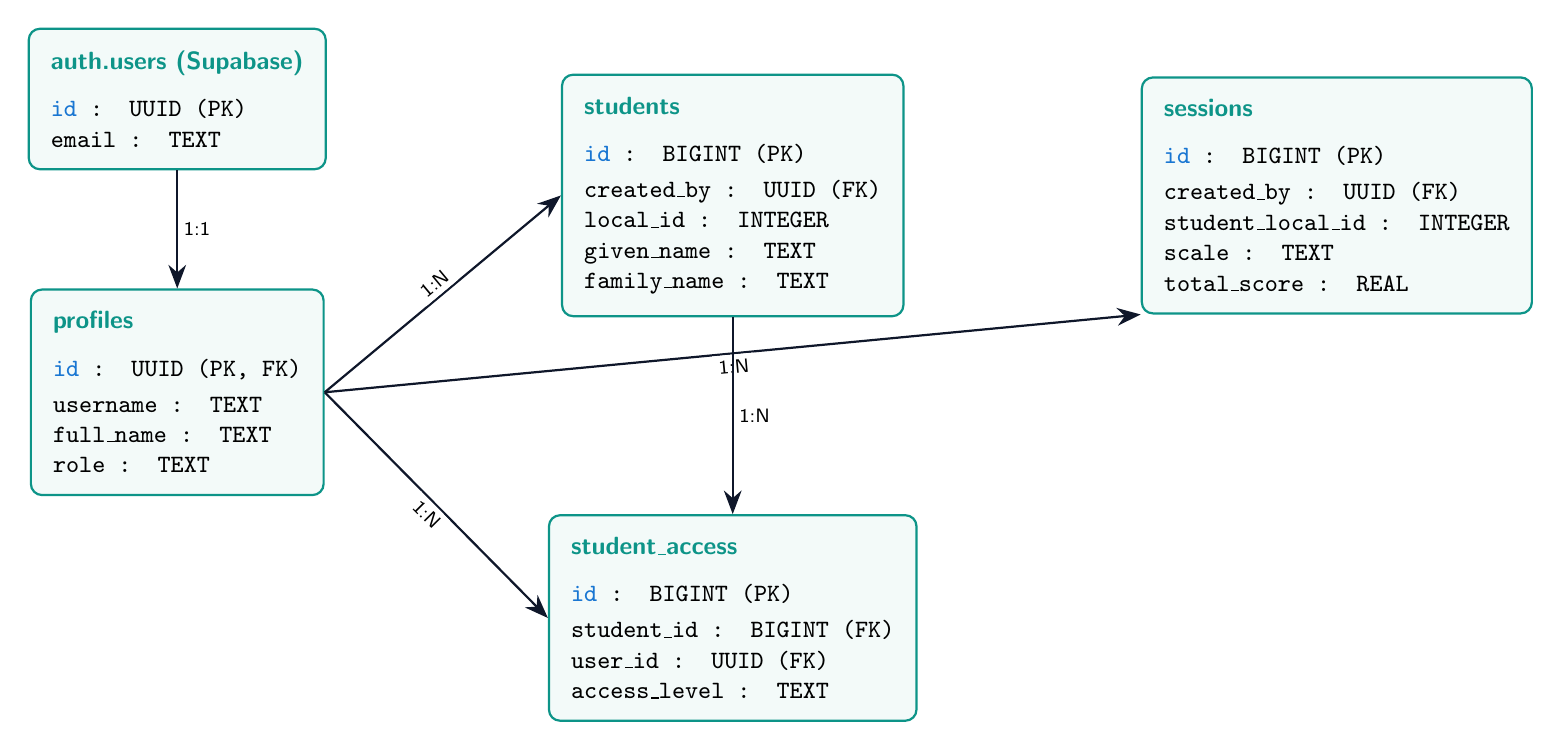
\begin{tikzpicture}[
    node distance=1.5cm and 3cm,
    entity/.style={
        draw=primaryteal, thick, fill=primaryteal!5,
        rectangle, rounded corners,
        inner sep=8pt, align=left,
        font=\small\ttfamily
    },
    rel/.style={
        -{Stealth[length=3mm]}, thick, draw=darkbg
    },
    lbl/.style={
        fill=white, font=\scriptsize\sffamily, inner sep=2pt
    }
]

% auth.users
\node[entity] (auth) {
    \textbf{\textsf{\color{primaryteal}auth.users (Supabase)}}\\[6pt]
    \textcolor{sqlblue}{id} : UUID (PK)\\
    email : TEXT
};

% profiles
\node[entity, below=of auth] (profiles) {
    \textbf{\textsf{\color{primaryteal}profiles}}\\[6pt]
    \textcolor{sqlblue}{id} : UUID (PK, FK)\\[2pt]
    username : TEXT\\
    full\_name : TEXT\\
    role : TEXT
};

% students
\node[entity, right=of profiles, yshift=2.5cm] (students) {
    \textbf{\textsf{\color{primaryteal}students}}\\[6pt]
    \textcolor{sqlblue}{id} : BIGINT (PK)\\[2pt]
    created\_by : UUID (FK)\\
    local\_id : INTEGER\\
    given\_name : TEXT\\
    family\_name : TEXT
};

% sessions
\node[entity, right=of students] (sessions) {
    \textbf{\textsf{\color{primaryteal}sessions}}\\[6pt]
    \textcolor{sqlblue}{id} : BIGINT (PK)\\[2pt]
    created\_by : UUID (FK)\\
    student\_local\_id : INTEGER\\
    scale : TEXT\\
    total\_score : REAL
};

% student_access
\node[entity, below=of students, yshift=-1cm] (studentaccess) {
    \textbf{\textsf{\color{primaryteal}student\_access}}\\[6pt]
    \textcolor{sqlblue}{id} : BIGINT (PK)\\[2pt]
    student\_id : BIGINT (FK)\\
    user\_id : UUID (FK)\\
    access\_level : TEXT
};

% Relationships
\draw[rel] (auth.south) -- node[lbl, right] {1:1} (profiles.north);
\draw[rel] (profiles.east) -- node[lbl, sloped, above] {1:N} (students.west);
\draw[rel] (profiles.east) -- node[lbl, sloped, below] {1:N} (sessions.south west);
\draw[rel] (profiles.east) -- node[lbl, sloped, below] {1:N} (studentaccess.west);
\draw[rel] (students.south) -- node[lbl, right] {1:N} (studentaccess.north);

\end{tikzpicture}
}
\caption{Supabase Cloud Entity-Relationship Diagram highlighting multi-role and access linking relationships.}
\end{figure}

% ============================================================================
\section{Offline-First Sync Engine}
% ============================================================================

The sync engine follows a \textbf{git-like model}: changes are committed locally to SQLite, queued for push, and synchronized with Supabase when connectivity is available. The architecture comprises three tightly coupled modules:

\subsection{Architecture Overview}

\begin{figure}[H]
\centering
\resizebox{0.85\textwidth}{!}{
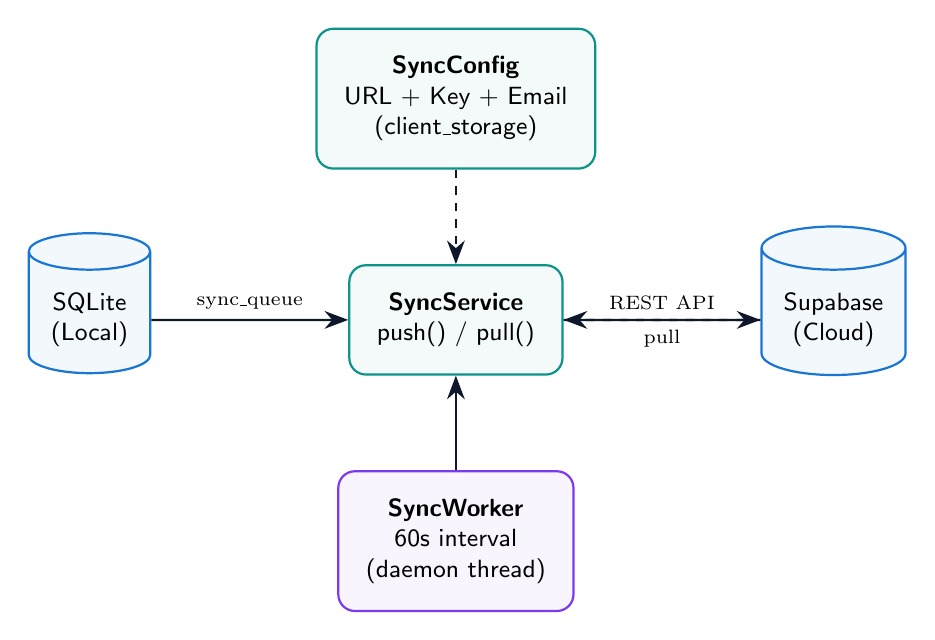
\begin{tikzpicture}[
    node distance=1.2cm and 2.5cm,
    box/.style={
        draw=primaryteal, thick, fill=primaryteal!5,
        rectangle, rounded corners=6pt,
        inner sep=10pt, align=center,
        font=\small\sffamily
    },
    worker/.style={
        draw=accentpurple, thick, fill=accentpurple!5,
        rectangle, rounded corners=6pt,
        inner sep=10pt, align=center,
        font=\small\sffamily
    },
    db/.style={
        draw=sqlblue, thick, fill=sqlblue!5,
        cylinder, shape border rotate=90,
        inner sep=8pt, align=center,
        font=\small\sffamily,
        aspect=0.3,
    },
    arr/.style={
        -{Stealth[length=3mm]}, thick, draw=darkbg
    },
]
\node[db] (sqlite) {SQLite\\(Local)};
\node[box, right=of sqlite] (syncengine) {\textbf{SyncService}\\push() / pull()};
\node[db, right=of syncengine] (supa) {Supabase\\(Cloud)};
\node[worker, below=of syncengine] (worker) {\textbf{SyncWorker}\\60s interval\\(daemon thread)};
\node[box, above=of syncengine] (config) {\textbf{SyncConfig}\\URL + Key + Email\\(client\_storage)};

\draw[arr] (sqlite) -- node[above, font=\scriptsize] {sync\_queue} (syncengine);
\draw[arr] (syncengine) -- node[above, font=\scriptsize] {REST API} (supa);
\draw[arr, dashed] (supa) -- node[below, font=\scriptsize] {pull} (syncengine);
\draw[arr] (worker) -- (syncengine);
\draw[arr, dashed] (config) -- (syncengine);
\end{tikzpicture}
}
\caption{Offline-first sync architecture. The SyncWorker daemon auto-syncs pending items every 60 seconds.}
\end{figure}

\subsection{SyncService — Core Engine}

The \texttt{SyncService} class (\texttt{sync\_service.py}, 557 lines) implements the full push/pull lifecycle:

\begin{itemize}[leftmargin=2em]
    \item \textbf{Push (Local $\rightarrow$ Cloud):} Reads unsynced items from \texttt{sync\_queue}, maps payloads to cloud schema columns, and upserts into Supabase using \texttt{(created\_by, local\_id)} as the conflict key. Supports \texttt{INSERT}, \texttt{UPDATE}, and soft-\texttt{DELETE} operations.
    \item \textbf{Pull (Cloud $\rightarrow$ Local):} Queries Supabase for records modified since the last pull timestamp (stored in \texttt{sync\_metadata}). Skips records that have pending local changes to prevent data loss. Handles both student and session tables.
    \item \textbf{Connectivity Check:} Validates connectivity by attempting a TCP connection to the Supabase host on port 443, with a fallback to Google DNS (\texttt{8.8.8.8:53}).
    \item \textbf{Full Sync:} Orchestrates push-then-pull with automatic profile upsert to satisfy foreign key constraints.
    \item \textbf{Cloud Restore:} Resets the last-pull timestamp and performs a full pull — used when a user logs in on a new device.
\end{itemize}

\subsection{SyncWorker — Background Thread}

The \texttt{SyncWorker} (\texttt{sync\_worker.py}) runs as a daemon thread with a configurable interval (default 60 seconds). It:

\begin{enumerate}[leftmargin=2em]
    \item Waits 5 seconds after app startup for full initialization
    \item Checks for pending items in the \texttt{sync\_queue}
    \item Verifies internet connectivity and authentication state
    \item Triggers a full sync cycle if conditions are met
    \item Sleeps in 1-second increments to allow quick shutdown
\end{enumerate}

\subsection{SyncConfig — Credential Management}

Supabase credentials are managed via Flet's \texttt{client\_storage} API, which provides persistent key--value storage per device. The configuration includes:

\begin{itemize}[leftmargin=2em]
    \item \texttt{supabase\_url}: Default project URL (hardcoded for convenience)
    \item \texttt{supabase\_key}: Anon key (safe to embed — RLS protects data)
    \item \texttt{cloud\_email}: Persisted for session restoration
    \item \texttt{cloud\_password}: \textit{Never persisted} — kept in-memory only during active sessions
\end{itemize}

\subsection{Cloud Account Restoration}

A critical edge case was addressed for clinical staff switching devices. If a user logs into a new device using an already registered email, the local SQLite database will be empty. The system now detects this, connects to Supabase, \textbf{restores the user's role and profile metadata}, and subsequently triggers a full sync to populate the device's local database.

% ============================================================================
\section{Authentication \& Session Management}
% ============================================================================

Security is implemented as a dual-layer system: \textbf{local authentication} (SQLite + PBKDF2) for offline access, and \textbf{cloud authentication} (Supabase Auth) for sync capabilities.

\subsection{Local Authentication}

The \texttt{AuthService} class (\texttt{auth\_service.py}, 269 lines) manages the full authentication lifecycle:

\begin{itemize}[leftmargin=2em]
    \item \textbf{Password Hashing:} Uses PBKDF2-SHA256 with 200,000 iterations and a random 16-byte salt. Stored as \texttt{pbkdf2\_sha256\$iterations\$salt\_b64\$digest\_b64}.
    \item \textbf{Session Persistence:} User sessions are stored in Flet's \texttt{client\_storage} using \texttt{auth\_user\_id} and \texttt{auth\_username} keys.
    \item \textbf{User Model:} The \texttt{AppUser} dataclass includes \texttt{username}, \texttt{password\_hash}, \texttt{full\_name}, \texttt{role}, \texttt{is\_active}, \texttt{email}, \texttt{cloud\_uid}, and \texttt{created\_at}.
\end{itemize}

\subsection{Cloud Authentication Integration}

When a user registers or logs in locally, the \texttt{AuthService} automatically:

\begin{enumerate}[leftmargin=2em]
    \item Registers with Supabase Auth (email + password + metadata)
    \item Creates/updates the \texttt{profiles} row with role and full name
    \item Stores the Supabase UUID (\texttt{cloud\_uid}) in the local database
    \item Persists a refresh token to \texttt{\textasciitilde/.gmfm\_app/.cloud\_token} for session restoration
\end{enumerate}

\subsection{New Device Account Recovery}

If a user attempts to log in on a new device where the local database is empty:

\begin{enumerate}[leftmargin=2em]
    \item The local lookup fails (no matching username)
    \item If the input contains ``@'', the system attempts a Supabase login
    \item On success, it fetches the cloud profile (name, role, email)
    \item Creates a new local \texttt{AppUser} with the restored credentials
    \item Triggers a full cloud-to-local data sync
\end{enumerate}

\begin{infobox}[Design Decision: Dual-Auth Architecture]
The dual-auth approach ensures the app works offline while enabling seamless multi-device sync. Local auth uses industry-standard PBKDF2; cloud auth leverages Supabase's JWT-based system. The two are linked via the \texttt{cloud\_uid} field.
\end{infobox}

% ============================================================================
\section{Role-Based Access Control (RBAC)}
% ============================================================================

Security and data privacy are paramount in clinical environments. We introduced a comprehensive Role-Based Access Control system enforced at both the UI (Route Guards) and Cloud (Row Level Security) levels.

The application now supports four distinct roles:

\begin{itemize}[leftmargin=2em]
    \item \textbf{Admin}: Full system access. Admins bypass Row Level Security constraints in the cloud and can manage all users and global app settings.
    \item \textbf{Teacher / Clinician}: Standard clinical access. Teachers can create and manage their own student profiles, conduct assessments, and view historical data for students they own.
    \item \textbf{Parent}: Limited read-only access. Parents are linked to specific students via the \texttt{student\_access} table. They can view the dashboard progress and detailed session histories for their children, but they are prevented from modifying data or conducting new assessments.
    \item \textbf{Sponsor}: Executive read-only access. Restricted entirely to the main dashboard. Sponsors can view high-level aggregate statistics (e.g., total sessions, average scores) but cannot access individual student profiles or session details.
\end{itemize}

\subsection{UI Route Guards}

The \texttt{GMFMApp.\_create\_view()} method actively intercepts navigation to enforce these rules. If a user attempts to access an unauthorized route, they are served a specialized ``Access Restricted'' view with a lock icon and descriptive message.

\begin{lstlisting}[style=python, caption={Role-based route guard logic (simplified)}]
# Sponsor: only dashboard (aggregate stats)
if user_role == "sponsor" and route != "/":
    return self._access_denied_view(route,
        "Sponsors can only view aggregate statistics")

# Parent: dashboard + session detail (read-only)
if user_role == "parent":
    allowed = route == "/" or route.startswith("/session")
              or route.startswith("/history")
    if not allowed:
        return self._access_denied_view(route,
            "Parents can view progress but cannot "
            "create or modify data")
\end{lstlisting}

\subsection{Login View with Role Selection}

The \texttt{LoginView} (\texttt{login\_view.py}, 268 lines) provides a polished registration flow with:

\begin{itemize}[leftmargin=2em]
    \item Visual role selection chips (Teacher, Admin, Parent, Sponsor) with distinct colors and icons
    \item Input validation (minimum 3-char username, 6-char password, valid email)
    \item Toggle between Sign In and Registration modes
    \item Footer badges indicating ``Offline First'', ``Encrypted'', and ``Cloud Sync'' capabilities
\end{itemize}

% ============================================================================
\section{Haptic Feedback Service}
% ============================================================================

To enhance the mobile assessment experience, a dedicated \texttt{HapticService} (\texttt{haptics.py}) was implemented using Flet's haptics API. The service provides six feedback patterns:

\begin{table}[H]
\centering
\begin{tabular}{@{}lll@{}}
\toprule
\textbf{Method}    & \textbf{Flet Type}           & \textbf{Use Case} \\
\midrule
\texttt{tap()}     & \texttt{LIGHT\_IMPACT}       & Button presses, selections \\
\texttt{select()}  & \texttt{SELECTION\_CLICK}     & Scoring items, toggles \\
\texttt{success()} & \texttt{MEDIUM\_IMPACT}       & Saves, completions \\
\texttt{heavy()}   & \texttt{HEAVY\_IMPACT}        & Celebrations, milestones \\
\texttt{warning()} & \texttt{MEDIUM\_IMPACT}       & Destructive action confirmations \\
\texttt{error()}   & \texttt{HEAVY\_IMPACT}        & Failed actions \\
\bottomrule
\end{tabular}
\caption{Haptic feedback patterns — optimized for linear vibration motors.}
\end{table}

All methods are wrapped in silent try/except blocks to ensure they degrade gracefully on platforms without haptic support (e.g., desktop, web).

% ============================================================================
\section{Adaptive UI Scaling (Android Accessibility)}
% ============================================================================

The \texttt{ui\_scale.py} module (125 lines) implements automatic UI scaling that respects Android's system-level text scale factor, ensuring the app is accessible to users with visual impairments.

\subsection{Scaling Algorithm}

\begin{enumerate}[leftmargin=2em]
    \item Read the \texttt{text\_scale\_factor} from Flet's \texttt{page.media} object
    \item Clamp the factor to a practical range: $[0.85, 1.60]$
    \item Recursively traverse the entire control tree of each view
    \item Scale numeric properties: \texttt{size}, \texttt{text\_size}, \texttt{icon\_size}, \texttt{width}, \texttt{height}, \texttt{stroke\_width}
    \item Scale compound spacing properties: \texttt{padding}, \texttt{margin}, \texttt{border\_radius} (handles both numeric and \texttt{ft.padding.only} objects)
    \item Track visited control IDs to prevent infinite loops in circular references
\end{enumerate}

The scaling is applied transparently via \texttt{apply\_android\_scale(page, view)} — called in \texttt{\_create\_scaled\_view()} for every route transition.

% ============================================================================
\section{Enhanced PDF Report Generation}
% ============================================================================

The \texttt{report\_service.py} (644 lines) implements a \textbf{three-tier fallback strategy} for PDF generation, ensuring reports can be generated on any platform:

\subsection{Backend Selection Waterfall}

\begin{figure}[H]
\centering
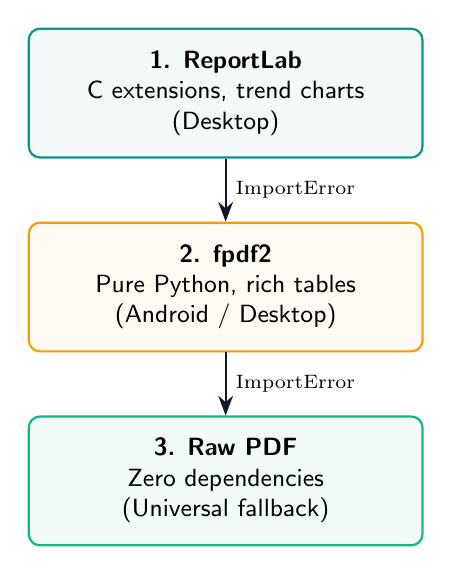
\begin{tikzpicture}[
    node distance=0.8cm,
    box/.style={
        draw=primaryteal, thick, fill=primaryteal!5,
        rectangle, rounded corners=4pt,
        inner sep=8pt, align=center,
        font=\small\sffamily, minimum width=5cm,
    },
    fallback/.style={
        draw=warnorange, thick, fill=warnorange!5,
        rectangle, rounded corners=4pt,
        inner sep=8pt, align=center,
        font=\small\sffamily, minimum width=5cm,
    },
    last/.style={
        draw=succegreen, thick, fill=succegreen!5,
        rectangle, rounded corners=4pt,
        inner sep=8pt, align=center,
        font=\small\sffamily, minimum width=5cm,
    },
    arr/.style={
        -{Stealth[length=2.5mm]}, thick, draw=darkbg
    },
]
\node[box] (rl) {\textbf{1. ReportLab}\\C extensions, trend charts\\(Desktop)};
\node[fallback, below=of rl] (fpdf) {\textbf{2. fpdf2}\\Pure Python, rich tables\\(Android / Desktop)};
\node[last, below=of fpdf] (raw) {\textbf{3. Raw PDF}\\Zero dependencies\\(Universal fallback)};

\draw[arr] (rl) -- node[right, font=\scriptsize] {ImportError} (fpdf);
\draw[arr] (fpdf) -- node[right, font=\scriptsize] {ImportError} (raw);
\end{tikzpicture}
\caption{PDF generation fallback waterfall. Each backend produces a complete GMFM score sheet.}
\end{figure}

\subsection{Raw PDF Engine}

The zero-dependency fallback (\texttt{\_generate\_raw\_pdf}) is a custom PDF renderer built using only Python builtins. It features:

\begin{itemize}[leftmargin=2em]
    \item \textbf{\_PdfPage class:} Accumulates PDF drawing commands (graphics + text) for each page
    \item Proportional Helvetica text rendering with approximate character widths ($\text{CHAR\_W} = 0.52$)
    \item Bordered table rows with shaded headers and full-width colored banners
    \item Automatic page breaks with re-printed domain headers on continuation pages
    \item Multi-page assembly with proper cross-reference tables and PDF 1.4 compliance
\end{itemize}

Each backend generates the same report structure:
\begin{enumerate}[leftmargin=2em]
    \item Student information header
    \item Total score highlight banner (teal background, white text)
    \item Domain summary table (5 domains with percentage and item counts)
    \item Detailed item-by-item score sheets per domain (columns: \#, Description, 0, 1, 2, 3, NT)
    \item Session notes (if any)
\end{enumerate}

% ============================================================================
\section{DOCX Import Pipeline}
% ============================================================================

The \texttt{docx\_import\_service.py} (371 lines) provides a complete pipeline for importing legacy GMFM assessment data from DOCX files — the format commonly used in clinical settings.

\subsection{Parser Architecture}

\begin{itemize}[leftmargin=2em]
    \item Uses \texttt{python-docx} with lazy import (graceful failure on Android)
    \item Iterates document body elements in order using \texttt{\_iter\_block\_items()} (paragraphs and tables)
    \item Extracts student metadata from paragraph text (name, assessment date, evaluator)
    \item Parses GMFM-88 scores from table rows, mapping item numbers to score values (0--3 or NT)
\end{itemize}

\subsection{Multi-Session Detection}

A single DOCX file may contain multiple assessment sessions for the same student. The parser detects session boundaries by:

\begin{enumerate}[leftmargin=2em]
    \item A new ``Assessment Date'' paragraph appearing after scores have been collected
    \item A duplicate item number appearing in the score table (e.g., Item \#1 repeated)
\end{enumerate}

Each detected session is output as a separate \texttt{ImportedAssessment} dataclass.

\subsection{Database Integration}

The \texttt{import\_assessment\_to\_db()} function handles:

\begin{itemize}[leftmargin=2em]
    \item Student deduplication by matching \texttt{given\_name} and \texttt{family\_name}
    \item Automatic student creation if no match is found
    \item Session creation with computed total scores
    \item Integration with the sync queue for cloud push
\end{itemize}

\begin{warnbox}[Platform Limitation]
DOCX import is only available on desktop platforms. On Android/iOS, \texttt{python-docx} is not bundled and the import raises a descriptive \texttt{ImportError}.
\end{warnbox}

% ============================================================================
\section{Data Security}
% ============================================================================

The \texttt{security.py} module implements a \texttt{SecurityProvider} class that provides field-level encryption using \texttt{Fernet} symmetric encryption (from the \texttt{cryptography} library):

\begin{itemize}[leftmargin=2em]
    \item \textbf{Key Resolution:} Environment variable $\rightarrow$ local file (\texttt{.gmfm\_key}) $\rightarrow$ auto-generate
    \item \textbf{Encrypt/Decrypt:} Optional per-field encryption for sensitive data before SQLite storage
    \item \textbf{Graceful Degradation:} If \texttt{cryptography} is not installed, the provider operates as a pass-through (no encryption)
\end{itemize}

% ============================================================================
\section{Animated Splash Screen}
% ============================================================================

The application features a branded splash screen with an animated logo sequence, implemented differently for mobile and desktop:

\subsection{Desktop Flow}

\begin{enumerate}[leftmargin=2em]
    \item Display splash container with Logo 1 at full opacity and Logo 2 hidden
    \item After 1.5 seconds: crossfade (Logo 1 $\rightarrow$ Logo 2) using Flet's \texttt{animate\_opacity} (500ms, ease-in-out)
    \item In parallel: initialize the database in a background thread
    \item After 1.5 seconds: wait for database thread completion (up to 15s timeout)
    \item Fade out entire splash (600ms ease-in-out)
    \item Clear splash controls and launch \texttt{GMFMApp}
\end{enumerate}

\subsection{Mobile Flow}

On Android/iOS, the splash is shown by \texttt{src/main.py} before the Flet engine fully initializes. The \texttt{gmfm\_app.main.main()} function detects the mobile platform and directly initializes the database and \texttt{GMFMApp} — the splash remains visible until \texttt{page.go("/")} is called.

\subsection{Splash Assets}

Logo images are embedded as base64-encoded constants in \texttt{splash\_assets.py} (1,055 KB). This avoids file-path issues on Android where the asset directory structure differs from desktop.

% ============================================================================
\section{Local Database Migrations}
% ============================================================================

The SQLite schema (\texttt{database.py}, 248 lines) uses a migration-friendly approach: each migration is wrapped in a try/except for \texttt{sqlite3.OperationalError} (column/table already exists), ensuring the app can be upgraded in-place without data loss.

\subsection{Migration History}

\begin{table}[H]
\centering
\begin{tabular}{@{}lL{9cm}@{}}
\toprule
\textbf{Migration} & \textbf{Description} \\
\midrule
M1 & Rename \texttt{patients} table to \texttt{students} \\
M2 & Add \texttt{notes} column to \texttt{sessions} \\
M3 & Add \texttt{role}, \texttt{is\_active} columns to \texttt{app\_users} \\
M4 & Rename \texttt{patient\_id} to \texttt{student\_id} in sessions \\
M5 & Add \texttt{email}, \texttt{cloud\_uid} columns to \texttt{app\_users} \\
M6 & Add \texttt{user\_id} column to \texttt{students} and \texttt{sessions} \\
M7 & Rename legacy \texttt{clinician} role to \texttt{teacher} \\
M8 & Create \texttt{sync\_queue} and \texttt{sync\_metadata} tables \\
M9 & Create \texttt{student\_access} table (parent/sponsor linking) \\
\bottomrule
\end{tabular}
\caption{SQLite migration history — applied automatically on app startup.}
\end{table}

% ============================================================================
\section{Navigation \& View Management}
% ============================================================================

The main application (\texttt{main.py}, 668 lines) implements a robust navigation system:

\begin{itemize}[leftmargin=2em]
    \item \textbf{View Stack:} Uses Flet's \texttt{page.views} list as a navigation stack. Forward navigation appends; back navigation pops.
    \item \textbf{Concurrency Guard:} A \texttt{\_nav\_lock} boolean prevents concurrent navigation events (fixes ``back too fast = blank screen'' bug).
    \item \textbf{Route History:} Maintains a bounded history (\texttt{max 20}, trimmed to last 10) for reliable back navigation.
    \item \textbf{Authentication Guard:} All routes except \texttt{/login} require authentication. Unauthenticated users are redirected to the login view.
    \item \textbf{Android Back Button:} The \texttt{view\_pop} handler supports Android's gesture-based back navigation, cleaning up stale overlays to prevent memory leaks.
    \item \textbf{Error Recovery:} All navigation paths are wrapped in try/except blocks. Failures produce a styled error view with stack trace rather than crashing the app.
\end{itemize}

\subsection{Route Map}

\begin{table}[H]
\centering
\begin{tabular}{@{}lll@{}}
\toprule
\textbf{Route} & \textbf{View} & \textbf{Roles Allowed} \\
\midrule
\texttt{/} & DashboardView & All \\
\texttt{/login} & LoginView & Public \\
\texttt{/student?id=\{id\}} & StudentView & Admin, Teacher \\
\texttt{/scoring?student\_id=\{id\}} & ScoringView & Admin, Teacher \\
\texttt{/history?student\_id=\{id\}} & SessionHistoryView & Admin, Teacher, Parent \\
\texttt{/session?session\_id=\{id\}} & SessionDetailView & Admin, Teacher, Parent \\
\texttt{/compare?session1=\{id\}\&session2=\{id\}} & CompareView & Admin, Teacher \\
\texttt{/settings} & SettingsView & Admin, Teacher \\
\bottomrule
\end{tabular}
\caption{Application route map with role-based access restrictions.}
\end{table}

% ============================================================================
\section{Standalone Windows Deployment}
% ============================================================================

To facilitate easy distribution in clinical environments where installing Python is not feasible, the deployment pipeline was finalized to include a bundled \textbf{Windows Executable (.exe)}.

Using \texttt{PyInstaller} and a custom \texttt{MotorMeasure\_Pro.spec} file, all required dependencies—including the \texttt{flet} engine, \texttt{supabase} client, \texttt{fpdf2} report generator, and \texttt{python-docx} import utilities—are now compiled into a standalone, portable binary. This effectively closes the loop on distribution, making MotorMeasure Pro a true plug-and-play solution for desktop environments.

% ============================================================================
\section{Complete Commit History}
% ============================================================================

The following table presents the full Git commit history of the project, organized chronologically across seven development phases.

\begin{longtable}{@{}C{1.2cm}L{2.2cm}L{2.5cm}L{7cm}@{}}
\toprule
\textbf{Hash} & \textbf{Date} & \textbf{Message} & \textbf{Key Changes} \\
\midrule
\endfirsthead
\toprule
\textbf{Hash} & \textbf{Date} & \textbf{Message} & \textbf{Key Changes} \\
\midrule
\endhead
\bottomrule
\endfoot

\multicolumn{4}{l}{\textit{\textbf{Phase 1 — Foundation (Nov 2025)}}} \\
\midrule
\texttt{375251d} & 2025-11-17 & Initial commit & Core GMFM-88 scoring engine, SQLite database, dashboard, student management \\
\texttt{edeff63} & 2025-11-22 & some\_updates & Initial UI refinements and data model adjustments \\
\texttt{2f050de} & 2025-11-22 & ui\_changes & Layout and styling improvements \\

\midrule
\multicolumn{4}{l}{\textit{\textbf{Phase 2 — UI \& Framework (Dec 2025)}}} \\
\midrule
\texttt{6da6253} & 2025-11-28 & some\_changes & View-level adjustments \\
\texttt{b3be147} & 2025-12-07 & new flet & Upgraded Flet framework version \\
\texttt{48f6984} & 2025-12-07 & changes & Post-upgrade compatibility fixes \\
\texttt{061acaa} & 2025-12-08 & ui\_improvements & Polished scoring and session views \\
\texttt{fbc7656} & 2025-12-08 & del & Cleanup of deprecated files \\
\texttt{d0535d7} & 2025-12-08 & ando & Android platform adaptation begins \\
\texttt{0d8e6c3} & 2025-12-09 & needs to be fixed & Identified Android-specific issues \\
\texttt{8763df8} & 2025-12-10 & haptics & Added HapticService with 6 feedback patterns \\

\midrule
\multicolumn{4}{l}{\textit{\textbf{Phase 3 — Data Import (Jan 2026)}}} \\
\midrule
\texttt{8a530c2} & 2026-01-05 & changes\_to\_add\_DOCX & DOCX import service, python-docx integration \\
\texttt{0a97b29} & 2026-01-12 & changes & Refinements to import pipeline \\
\texttt{a576dd5} & 2026-01-12 & ignores & Updated .gitignore for build artifacts \\
\texttt{3b42538} & 2026-01-24 & Update instructions\_data.json & GMFM-88 item instructions data update \\

\midrule
\multicolumn{4}{l}{\textit{\textbf{Phase 4 — Android \& Reports (Feb--Mar 2026)}}} \\
\midrule
\texttt{6123f95} & 2026-02-28 & uodate\_yeah & Cross-platform updates, chart service improvements \\
\texttt{0e16d4b} & 2026-03-02 & android\_fixed & Resolved Android platform crashes \\
\texttt{9544430} & 2026-03-02 & android\_fixed & Additional Android stability fixes \\
\texttt{71e6877} & 2026-03-02 & optimised & Repository pattern expansion, session view optimization \\
\texttt{dcb9b47} & 2026-03-02 & final? & Report service rewrite (fpdf2 + raw PDF), 540-line expansion \\
\texttt{cfeed0e} & 2026-03-02 & logo\_added & App logo integration, branding updates \\
\texttt{942e0c8} & 2026-03-02 & things\_done & Settings view expansion, theme persistence \\

\midrule
\multicolumn{4}{l}{\textit{\textbf{Phase 5 — Auth \& Login (Mar 2026)}}} \\
\midrule
\texttt{483cd11} & 2026-03-16 & 0.0.3, login & Login view, AuthService (PBKDF2), splash screen, UI scale service, 10,992 insertions \\

\midrule
\multicolumn{4}{l}{\textit{\textbf{Phase 6 — Cloud Sync (Apr 2026)}}} \\
\midrule
\texttt{30cfa50} & 2026-04-19 & login & SyncService, SyncWorker, SyncConfig, Supabase schema, development docs, 3,500 insertions \\
\texttt{e0ae73a} & 2026-04-19 & asdasd & Cloud auth refinements, DOCX import with user scoping \\
\texttt{f83ab76} & 2026-04-19 & ssss & Sync service bugfixes, requirements update \\

\end{longtable}

% ============================================================================
\section{Project Architecture Summary}
% ============================================================================

\begin{figure}[H]
\centering
\resizebox{\textwidth}{!}{
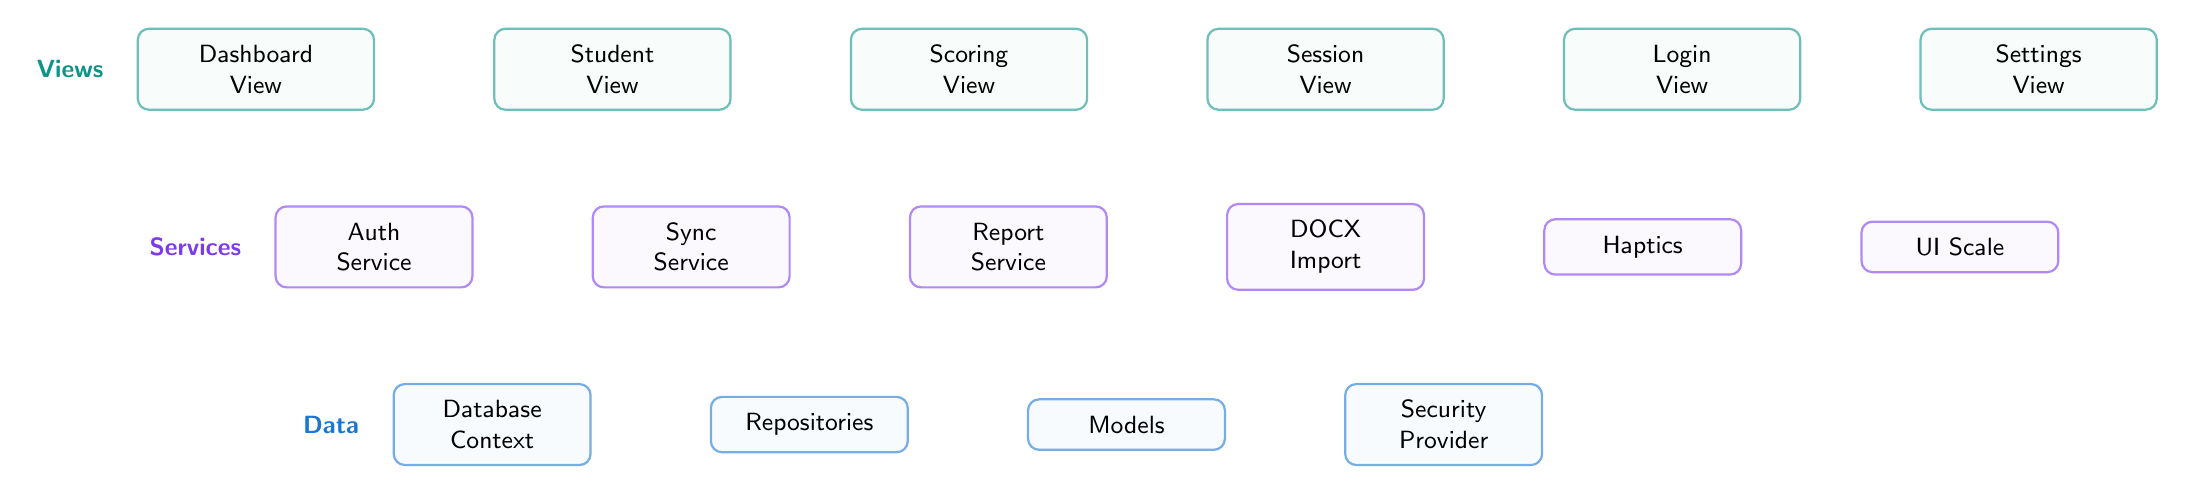
\begin{tikzpicture}[
    node distance=0.8cm and 1.5cm,
    layer/.style={
        draw=primaryteal!60, thick, fill=primaryteal!3,
        rectangle, rounded corners=4pt,
        inner sep=6pt, align=center,
        font=\small\sffamily, minimum width=3cm,
    },
    service/.style={
        draw=accentpurple!60, thick, fill=accentpurple!3,
        rectangle, rounded corners=4pt,
        inner sep=6pt, align=center,
        font=\small\sffamily, minimum width=2.5cm,
    },
    data/.style={
        draw=sqlblue!60, thick, fill=sqlblue!3,
        rectangle, rounded corners=4pt,
        inner sep=6pt, align=center,
        font=\small\sffamily, minimum width=2.5cm,
    },
]
% Views Layer
\node[layer] (dash) {Dashboard\\View};
\node[layer, right=of dash] (student) {Student\\View};
\node[layer, right=of student] (scoring) {Scoring\\View};
\node[layer, right=of scoring] (session) {Session\\View};
\node[layer, right=of session] (login) {Login\\View};
\node[layer, right=of login] (settings) {Settings\\View};

% Services Layer
\node[service, below=1.2cm of dash, xshift=1.5cm] (auth) {Auth\\Service};
\node[service, right=of auth] (sync) {Sync\\Service};
\node[service, right=of sync] (report) {Report\\Service};
\node[service, right=of report] (docx) {DOCX\\Import};
\node[service, right=of docx] (haptic) {Haptics};
\node[service, right=of haptic] (uiscale) {UI Scale};

% Data Layer
\node[data, below=1.2cm of auth, xshift=1.5cm] (db) {Database\\Context};
\node[data, right=of db] (repo) {Repositories};
\node[data, right=of repo] (models) {Models};
\node[data, right=of models] (security) {Security\\Provider};

% Labels
\node[left=0.3cm of dash, font=\small\bfseries\sffamily, color=primaryteal] {Views};
\node[left=0.3cm of auth, font=\small\bfseries\sffamily, color=accentpurple] {Services};
\node[left=0.3cm of db, font=\small\bfseries\sffamily, color=sqlblue] {Data};

\end{tikzpicture}
}
\caption{Three-layer architecture: Views $\rightarrow$ Services $\rightarrow$ Data.}
\end{figure}

\subsection{File Summary}

\begin{table}[H]
\centering
\begin{tabular}{@{}llr@{}}
\toprule
\textbf{Layer} & \textbf{File} & \textbf{Lines} \\
\midrule
\multirow{2}{*}{Core}
  & \texttt{main.py} & 668 \\
  & \texttt{splash\_assets.py} & $\sim$9,800 \\
\midrule
\multirow{6}{*}{Views}
  & \texttt{dashboard\_view.py} & 610 \\
  & \texttt{scoring\_view.py} & 660 \\
  & \texttt{session\_view.py} & 730 \\
  & \texttt{student\_view.py} & 240 \\
  & \texttt{settings\_view.py} & 490 \\
  & \texttt{login\_view.py} & 268 \\
\midrule
\multirow{7}{*}{Services}
  & \texttt{sync\_service.py} & 557 \\
  & \texttt{auth\_service.py} & 269 \\
  & \texttt{report\_service.py} & 644 \\
  & \texttt{docx\_import\_service.py} & 371 \\
  & \texttt{haptics.py} & 82 \\
  & \texttt{ui\_scale.py} & 125 \\
  & \texttt{security.py} & 92 \\
\midrule
\multirow{3}{*}{Data}
  & \texttt{database.py} & 248 \\
  & \texttt{repositories.py} & $\sim$450 \\
  & \texttt{models.py} & 109 \\
\bottomrule
\end{tabular}
\caption{Source file line counts by architectural layer.}
\end{table}

% ============================================================================
\section{Conclusion}
% ============================================================================

Over the course of seven development phases spanning November 2025 to June 2026, MotorMeasure Pro evolved from a standalone GMFM-88 scoring tool into a \textbf{full-stack, multi-user clinical assessment platform}. The key engineering achievements include:

\begin{enumerate}[leftmargin=2em]
    \item \textbf{Offline-First Architecture:} A git-like sync engine with local SQLite queue, background worker thread, and Supabase cloud backend ensures data is never lost — even without connectivity.
    \item \textbf{Enterprise Security:} Dual-layer authentication (PBKDF2 local + Supabase cloud), Row Level Security policies, and optional Fernet field-level encryption protect clinical data at rest and in transit.
    \item \textbf{Role-Based Access:} Four distinct user roles with UI route guards and cloud-enforced RLS policies ensure appropriate data visibility for clinicians, parents, sponsors, and administrators.
    \item \textbf{Cross-Platform Deployment:} The same codebase runs natively on Android (APK), Windows (standalone .exe), and desktop Python environments, with platform-specific adaptations for haptics, UI scaling, and asset loading.
    \item \textbf{Clinical Data Interoperability:} DOCX import for legacy data and multi-backend PDF export (ReportLab / fpdf2 / raw PDF) ensure seamless integration with existing clinical workflows.
\end{enumerate}

The total codebase now comprises over \textbf{15,000 lines of application code} across 20+ source files, with 25 tracked commits representing a structured progression from prototype to production-ready clinical software.

% ============================================================================
\end{document}
